\newpage

\section{РАЗРАБОТКА ПРОГРАММЫ}

\subsection{Выбор средств программирования}

Операционная система: \textbf{Ubuntu 20.10}.

Сервер: \textbf{LAMP} - Linux Apache2 MySQL PHP.

Блокнот: \textbf{VS Code 1.52.1}.

Браузер: \textbf{Mozilla Firefox 81.0.2}

\subsubsection{Установка LAMP}

Перед установкой LAMP обновляем список пакетов, используя команду \textbf{sudo apt update}. Устанавливаем LAMP командой \textbf{sudo apt install apache2 php libapache2-mod-php php-mysql mysql-server phpmyadmin}. Подробный скриншот на рисунке~\ref{fig:sudo-apt-install-apache2} (стр.~\pageref{fig:sudo-apt-install-apache2}).

\begin{figure}[!htp]
    \center{
        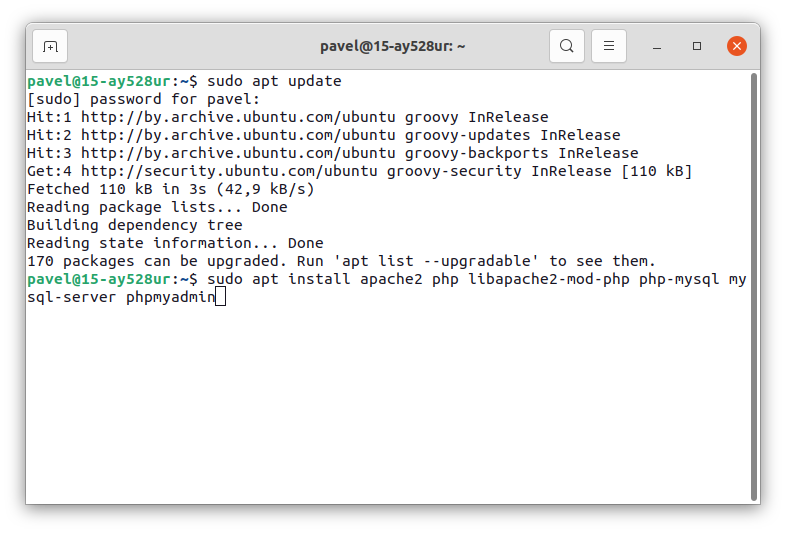
\includegraphics[width=16cm]
        {../_input/programDevelopment/install/sudo-apt-install-step-0.png}
    }
    \caption{Установка LAMP}
    \label{fig:sudo-apt-install-apache2}
\end{figure}

При установке пакетов нужно согласиться с установкой, нажав на клавишу <<Y>>, скриншот терминала на рисунке~\ref{fig:sudo-apt-install-apache2-step-1} (стр.~\pageref{fig:sudo-apt-install-apache2-step-1}).

\begin{figure}[!htp]
    \center{
        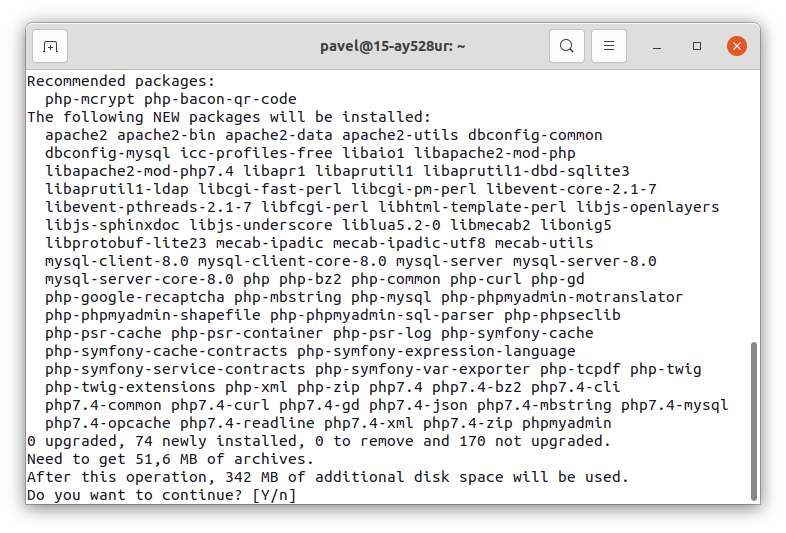
\includegraphics[width=16cm]
        {../_input/programDevelopment/install/sudo-apt-install-step-1.png}
    }
    \caption{Согласиться установить LAMP: нажать клавишу <<Y>>}
    \label{fig:sudo-apt-install-apache2-step-1}
\end{figure}

Выбираем флажки при установке, скриншот на рисунке~\ref{fig:sudo-apt-install-apache2-step-2} (стр.~\pageref{fig:sudo-apt-install-apache2-step-2}).

\begin{figure}[!htp]
    \center{
        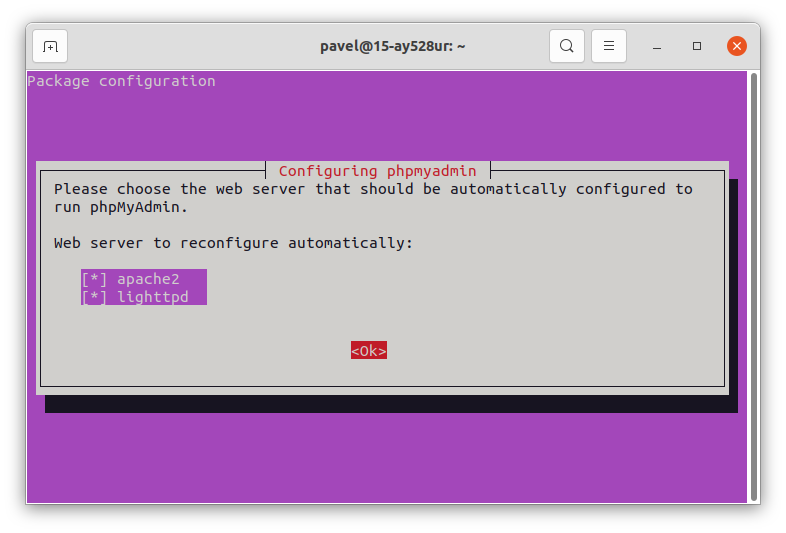
\includegraphics[width=16cm]
        {../_input/programDevelopment/install/sudo-apt-install-step-2.png}
    }
    \caption{Выбор флажков того, что установить, при установке LAMP}
    \label{fig:sudo-apt-install-apache2-step-2}
\end{figure}

Отвечаем на вопрос, скриншот на рисунке~\ref{fig:sudo-apt-install-apache2-step-3} (стр.~\pageref{fig:sudo-apt-install-apache2-step-3}).

\begin{figure}[!htp]
    \center{
        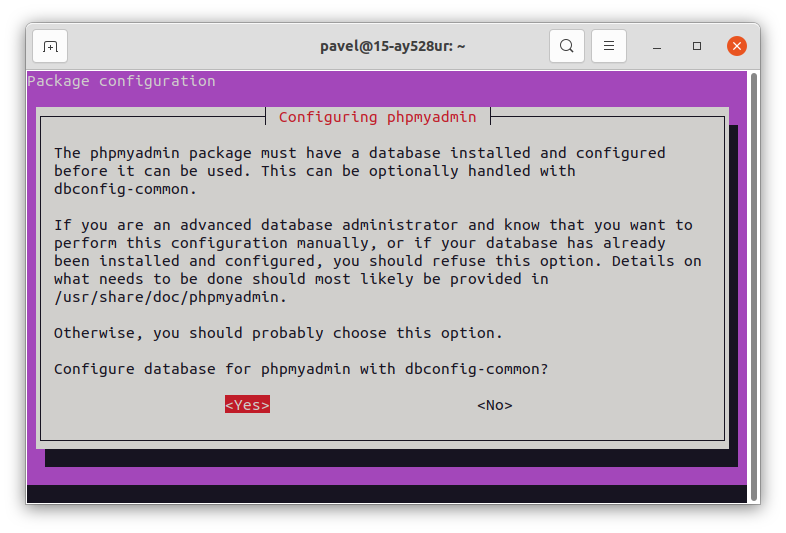
\includegraphics[width=16cm]
        {../_input/programDevelopment/install/sudo-apt-install-step-3.png}
    }
    \caption{Вопрос при установке LAMP}
    \label{fig:sudo-apt-install-apache2-step-3}
\end{figure}

После установки пакета <<phpmyadmin>> консоль предложит придумать пароль. Этот пароль будет пользователя под логином <<phpmyadmin>>, скриншот на рисунке~\ref{fig:sudo-apt-install-apache2-step-4} (стр.~\pageref{fig:sudo-apt-install-apache2-step-4}).

\begin{figure}[!htp]
    \center{
        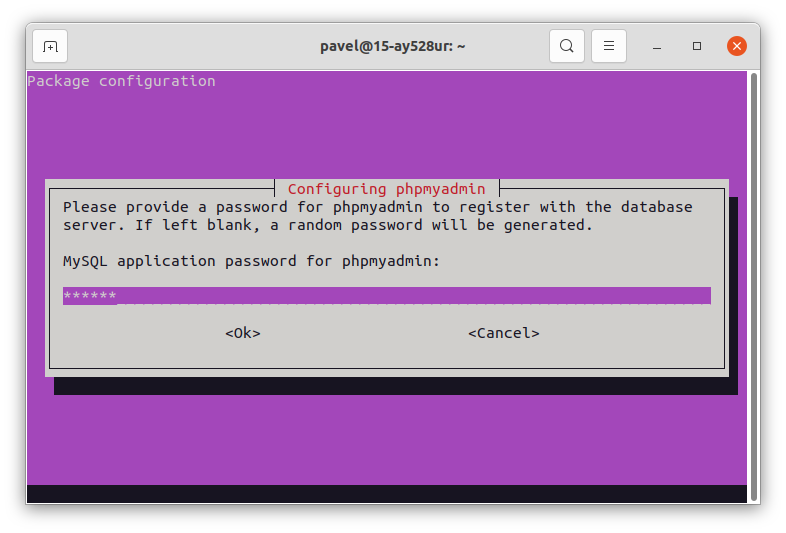
\includegraphics[width=16cm]{../_input/programDevelopment/install/sudo-apt-install-step-4.png}
    }
    \caption{Придумываем пароль для пользователя под логином <<phpmyadmin>>}
    \label{fig:sudo-apt-install-apache2-step-4}
\end{figure}

Как ввели пароль, то его нужно повторить. Повторяем пароль. Скришнот терминала на рисунке~\ref{fig:sudo-apt-install-apache2-step-5} (стр.~\pageref{fig:sudo-apt-install-apache2-step-5}).

\begin{figure}[!htp]
    \center{
        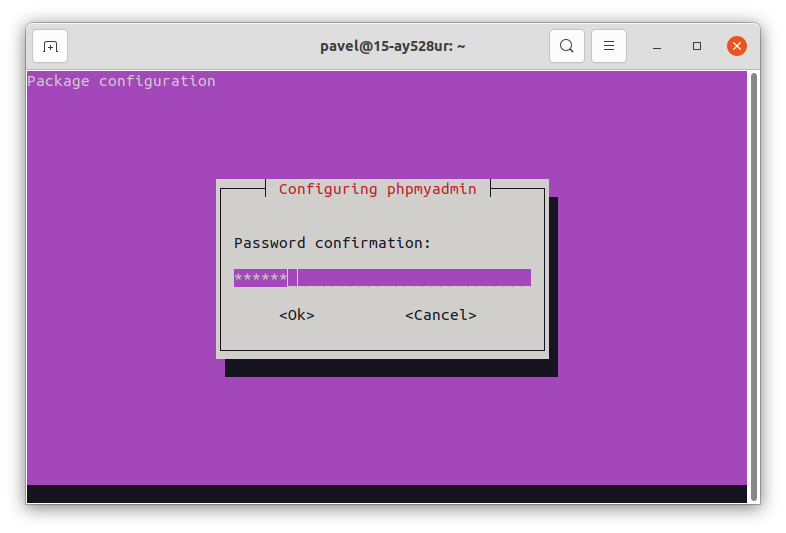
\includegraphics[width=16cm]{../_input/programDevelopment/install/sudo-apt-install-step-5.png}
    }
    \caption{Повторяем пароль для пользователя под логином <<phpmyadmin>>}
    \label{fig:sudo-apt-install-apache2-step-5}
\end{figure}

\begin{figure}[!htp]
    \center{
        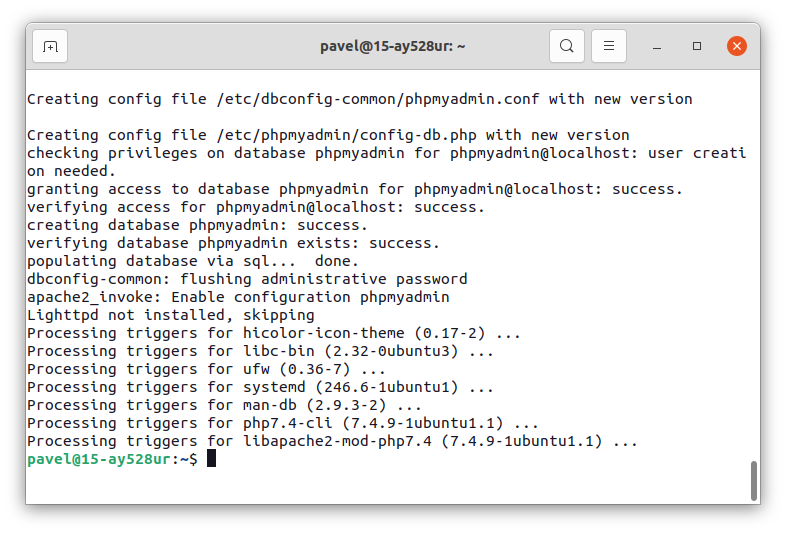
\includegraphics[width=16cm]{../_input/programDevelopment/install/sudo-apt-install-step-6.png}
    }
    \caption{Конец устаноки LAMP}
    \label{fig:sudo-apt-install-apache2-step-6}
\end{figure}

После установки Apache2, можем проверить сайт, вписав \textbf{localhost} в адресную строку браузера. Скриншот браузера с открытым сайтом на рисунке~\ref{fig:sudo-apt-install-apache2-step-7} (стр.~\pageref{fig:sudo-apt-install-apache2-step-7}).

\begin{figure}[!htp]
    \center{
        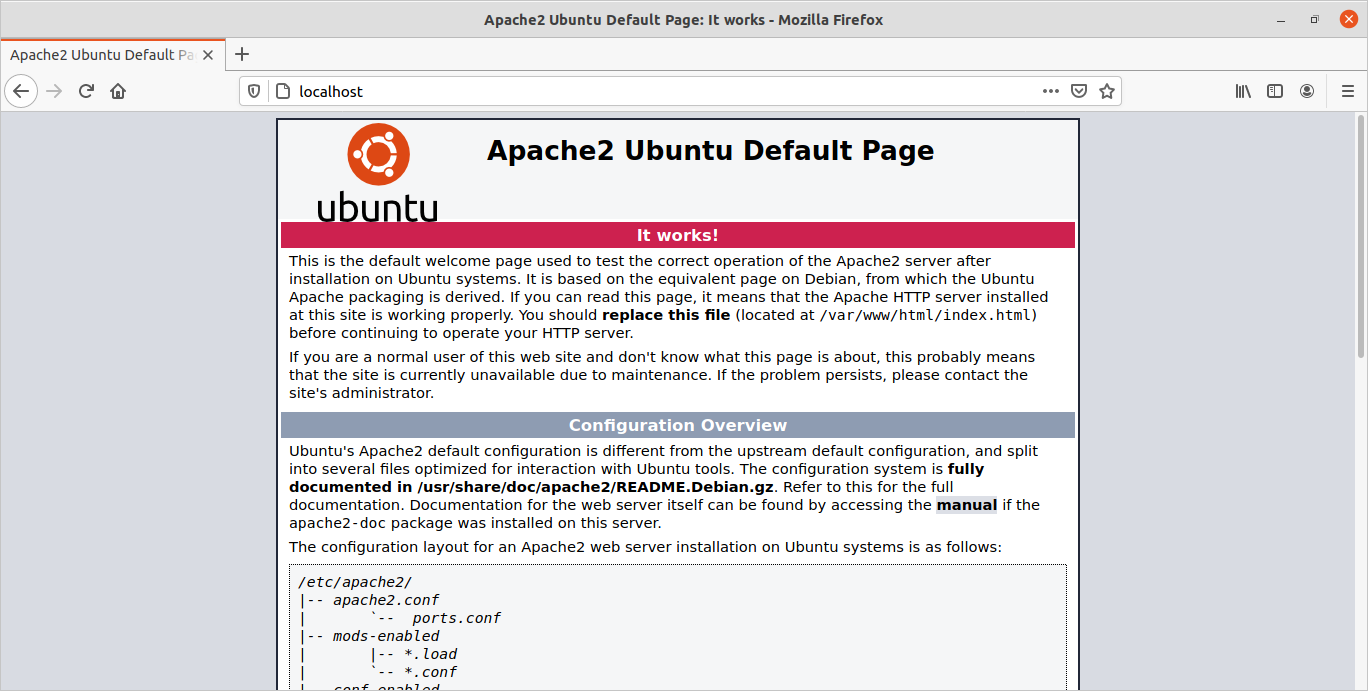
\includegraphics[width=16cm]{../_input/programDevelopment/install/sudo-apt-install-step-7.png}
    }
    \caption{Открываем сайт localhost в браузере}
    \label{fig:sudo-apt-install-apache2-step-7}
\end{figure}

\newpage

\subsubsection{Создание нового пользователя <<phpmyadmin>> с полными правами доступа}

Заходим на сраницу <<\textbf{localhost/phpmyadmin}>> под логином <<phpmyadmin>> и придуманым паролем - и видем, что мы не можем создавать базы данных. Для создания пользователя с такими привилегиями выполним скрипты:

\begin{verbatim}
sudo mysql -u root -p

CREATE USER 'admin'@'localhost' IDENTIFIED BY '111111';

GRANT ALL PRIVILEGES ON *.* TO 'admin'@'localhost' WITH GRAND OPTION;

FLUSH PRIVILEGES;
\end{verbatim}

Заходим на сраницу localhost/phpmyadmin под логином admin и паролем 111111 - и теперь можем создавать базу данных.

\subsubsection{Выделяем свой домен}

Создаем директорию для сайта

\begin{verbatim}
sudo mkdir /var/www/mysite
\end{verbatim}

Проект кладём в директорию /var/www/mysite.

Создаем файл с настройками на подобии стандартного:

\begin{verbatim}
sudo cp /etc/apache2/sites-available/000-default.conf
    /etc/apache2/sites-available/mysite.conf
\end{verbatim}

Открываем файл:

\begin{verbatim}
sudo nano /etc/apache2/sites-available/mysite.conf
\end{verbatim}

Добавляем домен и меняем путь:

\begin{verbatim}
ServerName mysite
DocumentRoot /var/www/mysite/src
\end{verbatim}

Для сохранения жмём "Ctrl" + "X", "y", "Enter".

Подлючаем файл с настройками:

\begin{verbatim}
sudo a2ensite mysite
\end{verbatim}

Перезагружаем Apache:

\begin{verbatim}
sudo systenctl reload apache2
\end{verbatim}

\subsubsection{Запускаем возможность работы файла настроек <<.htaccess>>}

В файле меняем строчку "AllowOverride None" на "AllowOverride All"

\begin{verbatim}
<Directory /var/www/>
        Options Indexes FollowSymLinks
#       AllowOverride None
        AllowOverride All
        Require all granted
</Directory>
\end{verbatim}

Теперь будет работать файл настроек ".htaccess". Создаем файл в директории

\begin{verbatim}
/var/www/mysite/src
\end{verbatim}

\subsubsection{Включаем debug mode PHP}

Чтобы отображались ошибки PHP заносим поля:

\begin{verbatim}
php_flag display_startup_errors on
php_flag display_errors on
php_flag html_errors on
\end{verbatim}

\hspace{0pt}\\

Задания выполнялись на языке программирования PHP. Верстка сайта велась по библиотеке Bootstrap. Для выполнения задачи на языке программирования PHP не потребовалось подключение библиотек. 

\hspace{0pt}

Среда разработки: Visual Studio Code.

\hspace{0pt}\\

ОС: Linux / Windows (при Windows можно использовать Open Server вместо LAMP)

\hspace{0pt}\\

В ходе написания проекта, проект был разбит на модули.

\hspace{0pt}\\

Использованы модули-сраницы: 

\begin{itemize}
    \item add
    \item show
\end{itemize}

\hspace{0pt}\\

Использованы модули-скрипты: 

\begin{itemize}
    \item form
\end{itemize}

\hspace{0pt}\\

Использованы многоразовые модули (для include): 

\begin{itemize}
    \item connect
    \item header
    \item menu
\end{itemize}

\newpage

\subsection{Разработка модулей}

\textbf{Модуль add}

\underline{Подключённые модули}:

\begin{enumerate}
    \item header
    \item menu
\end{enumerate}

\underline{Входные параметры}:

\begin{enumerate}
    \item Нет
\end{enumerate}

\underline{Назначение}: страница, которая имеет поля. После отправки, которые будет добавлены в базу MySQL.

\underline{Возвращаемые данные}: добавлены поля в базу данных MySQL.

\hspace{0pt}\\

% = = =

\textbf{Модуль show}

\underline{Подключённые модули}:

\begin{enumerate}
    \item header
    \item menu
    \item connect
\end{enumerate}

\underline{Входные параметры}:

\begin{enumerate}
    \item Нет
\end{enumerate}

\underline{Назначение}: страница, которая возвращает код HTML с удобочитаемой таблицой с даными.

\underline{Возвращаемые данные}: страница с отрисованной таблицей HTML.

\hspace{0pt}\\

% = = =

\textbf{Модуль form}

\underline{Подключённые модули}:

\begin{enumerate}
    \item connect
\end{enumerate}

\underline{Входные параметры}:

\begin{enumerate}
    \item model - модель (желаемый тип - строка)
    \item name - имя (желаемый тип - строка)
    \item onBox - количество в коробке (желаемый тип - не отрицательное целочисленное значение)
    \item weight - вес (желаемый тип - число с плавающей точкой)
    \item m3 - объем (желаемый тип - число с плавающей точкой)     
    \item series - серия (желаемый тип - строка) 
\end{enumerate}

\underline{Назначение}: скрипт, который принимает входный параметры по средствам POST запросов. Использует входные параметры для добавления в базу данных.

\underline{Возвращаемые данные}: данные появяться в базе MySQL. Сраница перенаправаться в корень.

\hspace{0pt}\\

% = = =

\textbf{Модуль connect}

\underline{Входные параметры}:

\begin{enumerate}
    \item site - сайт (желаемы тип - строка, например,  "localhost")
    \item userDB - логин в базе данных (желаемый тип - строка, например, "admin")
    \item passwordDB - пароль от базы данных (желаемый тип строка, например, "111111")
    \item database - имя базы данных (желаемый тип - строка, например, "productsdb")
    \item table - имя таблицы (желаемый тип - строка, например, "productstable")
\end{enumerate}

\underline{Назначение}: скрипт, который под входными данными подключится к базе данных.

\underline{Возвращаемые данные}: удачное/неудачное подключение к базе данных

\hspace{0pt}\\

% = = =

\textbf{Модуль header}

\underline{Входные параметры}:

\begin{enumerate}
    \item title - название страницы (желаемый тип - строка)
\end{enumerate}

\underline{Назначение}: страница с кодом HTML c заполненым тегом head.

\underline{Возвращаемые данные}: вставленый код HTML.

\hspace{0pt}\\

% = = =

\newpage

\textbf{Модуль menu}

\underline{Входные параметры}:

\begin{enumerate}
    \item нет
\end{enumerate}

\underline{Назначение}: страница с кодом HTML c заполненым меню.

\underline{Возвращаемые данные}: вставленый код HTML.

\hspace{0pt}\\

% = = =

\newpage